\chapter{System Architecture}
The proposed architecture of the system is discussed in
this section, which consists of the following components
(Figure 3.1).
\begin{figure}[htbp]
\centerline{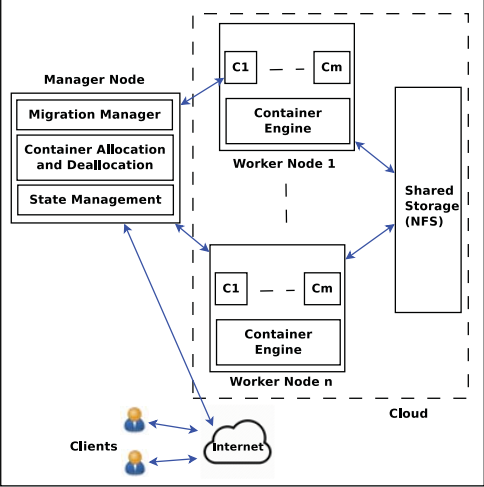
\includegraphics[width=0.5\textwidth]{fig1}}
\caption{ State transition diagram of a docker container}
\label{fig}
\end{figure}
\begin{enumerate}[i]
\item \textbf{Clients}: Clients send service request to the manager
node of the cloud data center.
\item \textbf{Manager Node}: The manager node is connected to all
the worker nodes of the cloud data center. The manager
node has a container allocation and deallocation module
to place the services in the cloud data center. This node
does the aggregation of the results. Also, the final result
is sent to the clients. We need to find the status of the
container state (active/idle). This work is performed by
the state management module. The container allocation
and deallocation module checkpoints the idle containers.
If the current server does not have sufficient resources,
we need to migrate the container to a new worker node.
This migration is performed by the migration manager
module of the manager node. State management module
is responsible for letting the migration manager module
know about the idle containers to be migrated at each
time instant.
\item \textbf{Cloud Worker Node}: The cloud worker node has
container engine (https://docs.docker.com/get-started/
overview/) to run different services as a container.
\item \textbf{Shared Storage using Network File System}: The cloud
worker nodes share a storage to save the state of the
checkpointed containers. This shared storage is designed
using NFS. NFS server is configured in a worker node
that needs to share its directory with other worker nodes.
NFS client is configured in the worker nodes that need
to access the NFS server’s directory.
\end{enumerate}
\begin{figure}[htbp]
\centerline{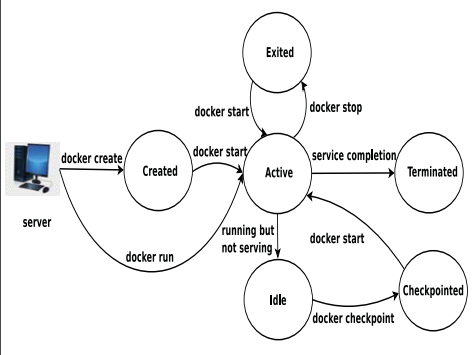
\includegraphics[width=0.7\textwidth]{fig2}}
\caption{ State transition diagram of a docker container}
\label{fig}
\end{figure}
The management of a container’s states is a very challenging
task as a container goes through many states in its lifecycle. We discuss the state transition of a docker container in
Figure 3.2. When a docker is running and serving the requests,
it goes to an active state. The docker container goes to an
idle state when it is running but not serving any requests.
Docker containers can be checkpointed to save the current
running state of the container. The docker container goes to
a checkpointed state when we save the running state of the
container. The checkpointed container can be resumed to make
it active again. After the complete service completion, the
docker container goes to a terminated state.

\section{Service State Management Of Containerized Applications}
Let us consider c containers and s servers present in the
system at a particular time instant. We denote \begin{math} S = \{ S\textsubscript{i} :   i \in (1,...,s) \} \end{math} and \begin{math} C\textsubscript{i} = \{C\textsubscript{j} : j \in (1,...,c)\}\end{math} as sets of cloud
data center servers and containers respectively.
\subsection{Average Startup Latency of the Services}
We need to start the checkpointed service whenever a
request comes. Therefore, the startup latency for the checkpointed container is defined as
\begin{align*} Startup\_latency\textsubscript{i} = Container\_resumption\_time\textsubscript{i}+
\\ Migration\_time\textsubscript{i}\end{align*}
where \begin{math} Container\_resumption\_time\textsubscript{i}\end{math} is the time taken by
the system to resume the container \begin{math} i \end{math} and \begin{math} Migration\_time\textsubscript{i} \end{math} is the communication time needed to transfer the state from
the source node to the destination node for the container \begin{math}i \end{math}. We define the startup latency for the new container as \begin{align*} Startup\_latency\textsubscript{i} = Container\_deployment\_time\textsubscript{i}\end{align*} where \begin{math} Container\_deployment\_time\textsubscript{i} \end{math} is the time taken by
the system to deploy the new container \begin{math} i \end{math}. \begin{math}Startup\_latency\textsubscript{i} \end{math} is the individual startup delay of a service \begin{math} i \end{math}. Therefore, the
average startup latency is defined as \begin{align*} Avg\textsubscript{startup\_latency} =\frac {\sum_{n=1}^{c} Startup\_latency\textsubscript{i}} {c} \end{align*}

\subsection{Average Response Time of the Services}
We define the response time of a service as
\begin{align*} Resp\_time\textsubscript{i} = Startup\_latency\textsubscript{i}+
 Service\_running\_time\textsubscript{i}\end{align*}
where \begin{math} Service\_running\_time\textsubscript{i}\end{math}
is the processing time taken
for a service in a server. Now, we define the average response
time of the services as,
\begin{align*} Avg\textsubscript{resp\_time} =\frac {\sum_{n=1}^{c} Resp\_time\textsubscript{i}} {c} ,\end{align*}
where \begin{math} Resp\_time\textsubscript{i}\end{math} is the individual response time of a service \begin{math} i \end{math}

\subsection{Constraints}
We define \begin{math} $$C_{j}^{CPU}$$ , $$C_{j}^{RAM}$$ ,  $$C_{j}^{BW}$$\end{math} and \begin{math}  $$C_{j}^{BW}$$\end{math} as the CPU, RAM, and bandwidth resources needed by a container \begin{math} C_j \end{math}
respectively. The available CPU, available RAM, and available bandwidth
of the server \begin{math} S\textsubscript{j}\end{math} are \begin{math}$$Re_{i}^{CPU}$$ , $$Re_{i}^{RAM}$$ ,  $$Re_{i}^{BW}$$ \end{math} respectively. We find \begin{math} k\end{math} servers \begin{math} K = (S\textsubscript{1}.....S\textsubscript{k})\end{math}  from the set of all servers \begin{math} S\end{math} where \begin{math} K \subseteq S\end{math} such that the following conditions are true. 
\begin{align*} \sum_{j=1}^{TC\textsubscript{i}} C_{j}^{CPU} \times x \textsubscript{i,j} \leq Re_{i}^{CPU} \times y\textsubscript{i} \numberthis \label{eqn} \end{align*}
\begin{align*} \sum_{j=1}^{TC\textsubscript{i}} C_{j}^{RAM} \times x \textsubscript{i,j} \leq Re_{i}^{RAM} \times y\textsubscript{i}\numberthis \label{eqn} \end{align*}
\begin{align*} \sum_{j=1}^{TC\textsubscript{i}} C_{j}^{BW} \times x \textsubscript{i,j} \leq Re_{i}^{BW} \times y\textsubscript{i} \numberthis \label{eqn} \end{align*}
where \begin{math} i = 1,....,s\end{math} and \begin{math} 0 \leq j \leq c\end{math}. We define \begin{math} x\textsubscript{i,j}\end{math} as the decision variable to denote if a container \begin{math} C_{j}\end{math} j has been placed in the server \begin{math} S_{j}\end{math}  Also, \begin{math} y_{i}\end{math} is the decision variable to denote if a server \begin{math} S_{i}\end{math} is used for placement or not. TC\textsubscript{i} is the total number of
containers present in the server  \begin{math} S_{i}\end{math}.
\begin{align*} \sum_{i=1}^{S} y\textsubscript{i} \geq 1 \numberthis \label{eqn} \end{align*} 
\begin{align*} \forall_{i,j}  x\textsubscript{i,j} \in \{0 , 1\} ; \forall_{j} y\textsubscript{i} \in \{0 , 1\} \numberthis \label{eqn} \end{align*} 
The following equation states that all the containers should
be deployed in the system. 
\begin{align*} \sum_{i=1}^{k} TC\textsubscript{i} =\mathopen | C \mathclose | \numberthis \label{eqn} \end{align*} 
where \begin{math}\mathopen | C \mathclose | \end{math} is the cardinality of the set \begin{math} C \end{math}.
We have another constraint that one container can be placed
in exactly one server.
\begin{align*}  \forall_{j} \sum_{i=1}^{k} x\textsubscript{i,j} =1 \numberthis \label{eqn} \end{align*} 

\subsection{Algorithm Design}
We propose a heuristic algorithm called Service Deployment
Algorithm to find a near optimal solution. Also, we present
Container Checkpointing Algorithm and Container Resumption Algorithm to checkpoint and resume the containers respectively. We discuss the algorithms below
\subsection{Service Deployment Algorithm}
We present the Service Deployment Algorithm in Algorithm 1. The inputs of the algorithm are container set (C) and
cloud server set (S). The output of the Consolidation ratio.
Our aim is to maximize the consolidation ratio. The checkpointed containers are deployed in the same server where it run
last time if the server is able to meet the resource requirement
(Eq. (1, 2, 3)). Otherwise, a new server is chosen to deploy
the checkpointed container. The proposed algorithm deploys
the containers in the selected server (Su). If the resource
requirement is not met for some containers, we find whether
a checkpoint in the selected server can give enough resources
for the container to be deployed. If a checkpoint can give
the required resources, we identify the idle containers in the selected server and checkpoint them. This approach frees up
more resources that can be allocated to the new containers.
Otherwise, a new server is chosen for checking if deployment
is possible or not. In this way, the consolidation ratio is
maximized by our proposed algorithm. 

\begin{algorithm}
\caption{Service Deployment Procedure}
\begin{algorithmic}[1]
\State \textbf{Input : } Container Set ($C), Cloud Server Set ($S)
\State \textbf{Output : } \begin{math}Consolidation\_ratio \end{math}
\Procedure{Deployment}{$C,S$}       
    \State Sort the containers in descending order of their
resource requirement and store in \begin{math}Sorted\_con\end{math};
\For{$all\ the\ containers\ in\  Sorted\_con$} \begin{math} servers\_not\_available = 0\end{math} \EndFor
    
    \If{$the\ deployment\ request\ is\ for\ a\ checkpointed\
container$} \State \begin{math}k = -1\end{math} 
\State /*\begin{math}S\_last\_run\_C\textsubscript{i}\end{math} is server where the checkpointed container run last time*/
\State \begin{math}S\textsubscript{u} = S\_last run\_C\textsubscript{i};\end{math}
\Else
\State \begin{math}k = 0;\end{math}
\State \begin{math}S\textsubscript{u} = S[k];\end{math}
    \EndIf

    \While{the resource requirement of container C\textsubscript{i}
is greater than  the resource available in
server S\textsubscript{u}} 
         \If{$checkpointing\ in\ server\ S\textsubscript{u}\ can\ deploy\
the\ container\ C\textsubscript{i}$} \State \begin{math}resource\_available\_in\_server =
Checkpoint\_idle\_containers(S\textsubscript{u});\end{math} 
\State Break the while loop

    \EndIf
 \If{$all\ servers\ are\ explored$} \State \begin{math}/*servers\_not\_available\end{math} is set
to 1 if no servers are
found for deployent*/
\State \begin{math}servers\_not\_available = 1\end{math}
\State Break the while loop
\Else
\State  \begin{math}k = k + 1\end{math}
\State \begin{math}S\textsubscript{u} = S[k];\end{math}
    \EndIf
 \If{$servers\_not\_available \neq 1$} \State Deploy the required container C\textsubscript{i} in the selected
server S\textsubscript{u};

\State Calculate \begin{math}Consolidation\_ratio \end{math}
    \EndIf

    \EndWhile  \label{loop}
\State \textbf{return} \begin{math}Consolidation\_ratio \end{math}
\EndProcedure

\end{algorithmic}
\end{algorithm}
\subsection{Container Resumption Algorithm}
In this subsection, we present the Container Resumption
Algorithm for resuming the idle containers. This algorithm
is described in Algorithm 3. The inputs of the algorithm
are the containers that need to be resumed (\begin{math}C\_resume \end{math}), the
container set (\begin{math}C\end{math}), and the cloud server set (\begin{math}S\end{math}). The output of
the algorithm is the \begin{math}Consolidation\_ratio \end{math}.



